\documentclass{article}
\usepackage{xeCJK,amsmath,geometry,float,graphicx,amssymb,zhnumber,booktabs,setspace,tasks,verbatim,amsthm,amsfonts,mathdots}
\usepackage{listings,xcolor}
\geometry{a4paper,scale=0.8}  
\renewcommand\arraystretch{2}
\title{图论作业 (第十周)}
\author{PB20000113孔浩宇}
\begin{document}
\maketitle
\section*{Ch6}
\subsection*{7.}
\begin{enumerate}
    \item [(1)]若图中存在两个奇数度的顶点$u,\ v$,则连接边$uv$,此时图为$Euler$图;若为$Euler$图,不操作
    \item [(2)]利用$Fleury$在图中寻找$Euler$回路,删除$uv$,即得到$Euler$迹。 (若原为$Euler$图,任删去一边)
\end{enumerate}

\subsection*{8.}
\begin{enumerate}
    \item []由EJ算法
    \item [(1)]图G中的奇度顶点集合为$V_0=\{v_1,\ v_2,\ v_3,\ v_4 \}$.
    \item [(2)]由$Dijkstra$算法得
    \[
        {dist}_{G}(v_1,\ v_2)=4, \quad {dist}_{G}(v_1,v_3)=5, \quad {dist}_{G}(v_1,\ v_4)=7.
    \]
    \[
        {dist}_{G}(v_2,\ v_3)=2, \quad {dist}_{G}(v_2,\ v_4)=5, \quad {dist}_{G}(v_3,\ v_4)=3.
    \]
    \item [(3)]构造加权完全图$K_4$
    \begin{figure*}[htbp]
        \centering
        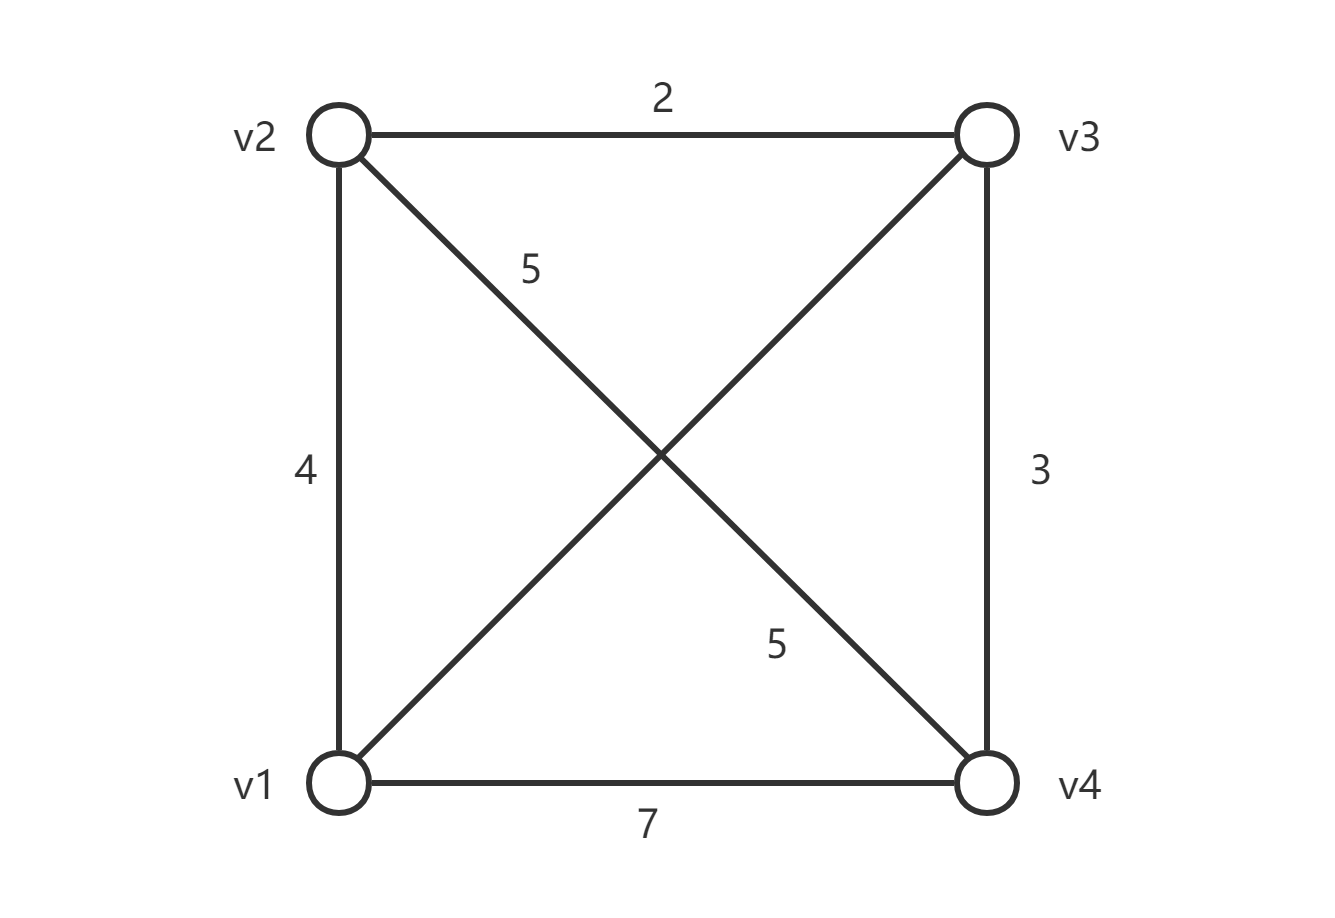
\includegraphics[scale=0.15]{t83.png}
    \end{figure*}
    \item [(4)]得到$K_4$中最小的完备匹配$\{v_1 v_2,\ v_3 v_4\}$,
    在$G$中将$v_1,\ v_2$间最短轨道$P(v_1 v_2)=v_1 v_7 v_2$及
    $v_3,\ v_4$间最短轨道$P(v_3 v_4)=v_3 v_4$重复一次得到$Euler$图$G *$.
    \item [(5)]在图$G*$中找到$Euler$回路即为最优投递路线。不妨取$v_5$为起点,可得一条$Euler$回路
    \[
        v_5\ v_1\ v_6\ 
        v_2\ v_3\ v_4\ 
        v_3\ v_7\ v_2\ 
        v_7\ v_1\ v_7\ 
        v_4\ v_5 .
    \]
\end{enumerate}

\subsection*{9.}
\begin{enumerate}
    \item [(1)]
    \begin{proof}
        不妨设二分图$G=(X,E,Y),\ X\cup Y=V(G),\ X\cap Y=\phi$.
        \[
            \begin{cases}
                \ \omega (G-X) & = \omega (Y) \leq |X|\\
                \\
                \ \omega (G-Y) & = \omega (X) \leq |Y|
            \end{cases}
            \xrightarrow[\omega(Y)=|Y|]{\omega(X)=|X|}
            \begin{cases}
                \ |X| &\leq |Y|\\
                \\
                \ |Y| &\leq |X|
            \end{cases}
            \Rightarrow\ 
            |X|=|Y|.
        \]
        显然$|G|=2|X|$为偶数,即证.
    \end{proof}
    \item [(2)]图6.27不是Hamilton图,因为$V(G)=\{v_0,\ v_1,\ v_6,\ v_7,\ v_{10} \}\cup \{v_2,\ v_3,\ v_4,\ v_5,\ v_8,\ v_9 \}$,
    为二分图,且$|G|=11$,故不是Hamilton图。
    \begin{figure*}[htbp]
        \centering
        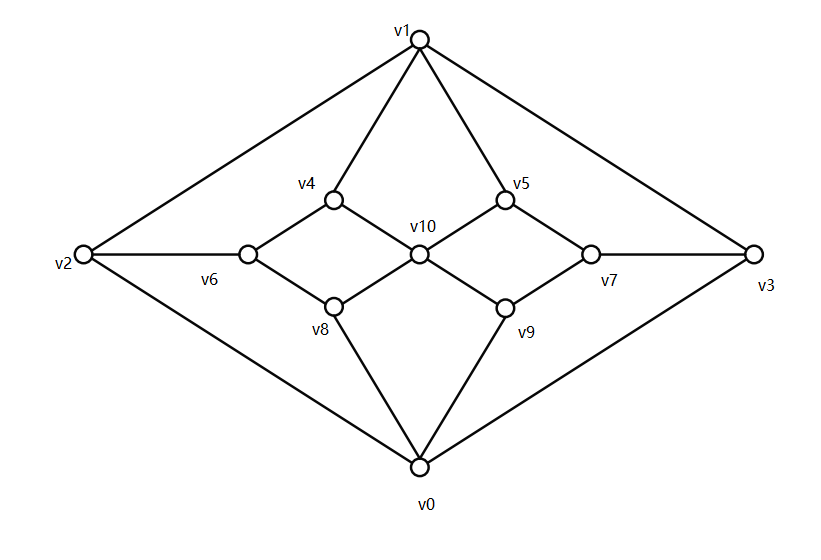
\includegraphics[scale=0.6]{t9.png}
    \end{figure*}
\end{enumerate}


\subsection*{12.}
\begin{enumerate}
    \item [(1)]$n$为奇数,如图
    \begin{figure*}[htbp]
        \centering
        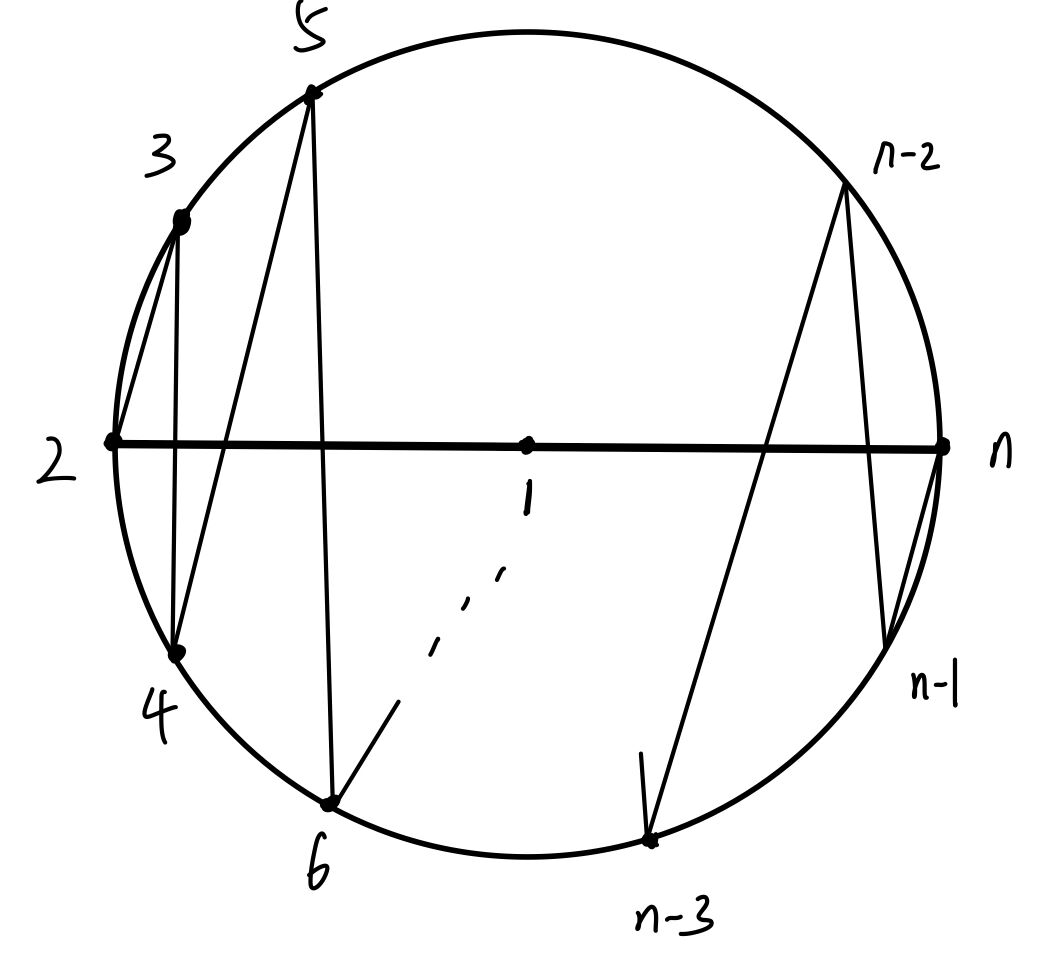
\includegraphics[scale=0.3]{t121.jpg}
    \end{figure*}

    显然,$(1,2,3,4,\ldots,n-2,n-1,n)$为$K_n$的一条$Hamilton$圈。现将圆周上的点的编号依次旋转$\displaystyle{\frac{2k\pi}{n-1}}\ (k=0,1,\ldots,\displaystyle{\frac{n-3}{2}})$,它们分布对于不重边的$Hamilton$圈:
    \begin{enumerate}
        \item []$(1,4,2,6,3,8,\ldots,n-1,n-4,n,n-2,1)$
        \item []$(1,6,4,8,2,10,\ldots,n,n-6,n-2,n-4,1)$
        \item []$\cdots$
        \item []$(1,n-1,n-3,n,n-5,n-2,\ldots,7,2,5,3,1)$
    \end{enumerate}
    \clearpage
    \item [(2)]$n$为偶数,如图 (在结点3,结点5的边上添加结点4)
    \begin{figure*}[htbp]
        \centering
        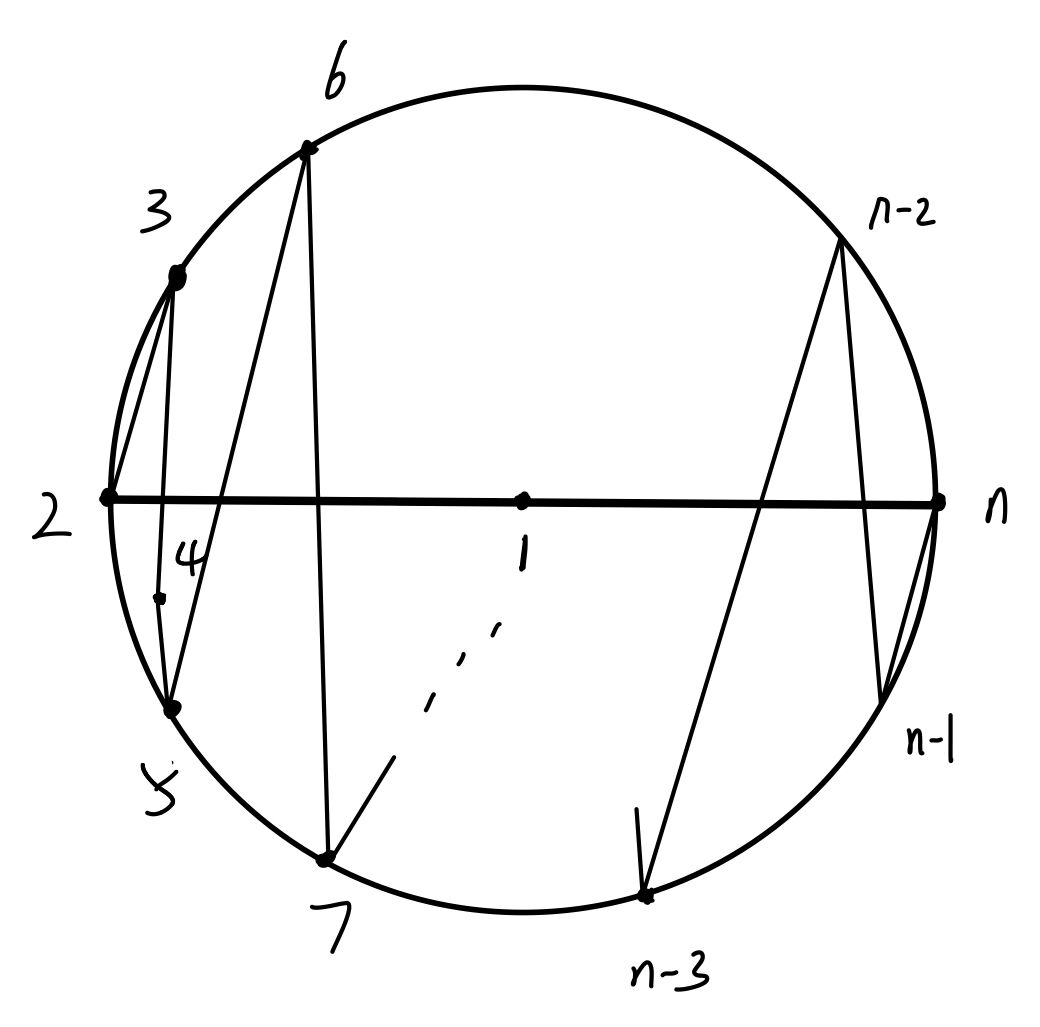
\includegraphics[scale=0.3]{t122.jpg}
    \end{figure*}

    显然,$(1,2,3,4,\ldots,n-2,n-1,n)$为$K_n$的一条$Hamilton$圈。现将圆周上的点的编号依次旋转$\displaystyle{\frac{2k\pi}{n-2}}\ (k=0,1,\ldots,\displaystyle{\frac{n-4}{2}})$,它们分布对于不重边的$Hamilton$圈:
    \begin{enumerate}
        \item []$(1,5,2,4,7,3,\ldots,n-1,n-4,n,n-2,1)$
        \item []$(1,7,5,4,9,2,\ldots,n,n-6,n-2,n-4,1)$
        \item []$\cdots$
        \item []$(1,n-1,n-3,4,n,n-5,\ldots,8,2,6,3,1)$
    \end{enumerate}
\end{enumerate}
综上,$K_n$共有$\left[\displaystyle{\frac{n-1}{2}}\right]$个不重边的$Hamilton$圈。

\subsection*{17.}
\begin{proof}
    \begin{enumerate}
        \item []
        \item [(1)]假设存在$u,\ v\in V(G)$,使得
        \[
            \deg (u) +\deg (v) \leq \nu-1
        \]
        取$G'=G-\{u,\ v\}$,此时有
        \begin{align*}
            |E(G')|&\geq m-(\nu-1)\\
            &=\displaystyle{\frac{1}{2}}(\nu -1)(\nu -2)+2 -(\nu -1)\\
            &=\displaystyle{\frac{1}{2}}(\nu -2)(\nu -3)+1\\
            &> |E(K_{\nu -2})|.
        \end{align*}
        显然矛盾,即$\forall\ u,\ v\in V(G)$,有
        \[
            \deg (u)+\deg (v)\geq \nu
            \ \Rightarrow
            \ G\mbox{为}Hamilton\mbox{图}.
        \]
        \item [(2)]比如构造图$G=K_{\nu -1} + u$,连接$u$与$K_n$中任一点,此时$m=\displaystyle{\frac{1}{2}}(\nu -1)(\nu -2)+1$,但显然不是$Hamilton$图.
    \end{enumerate}
\end{proof}
\clearpage
\subsection*{19.}不妨设这6个人顺时针依次为A,B,C,D,E,F,解法如图
\begin{figure*}[htbp]
    \centering
    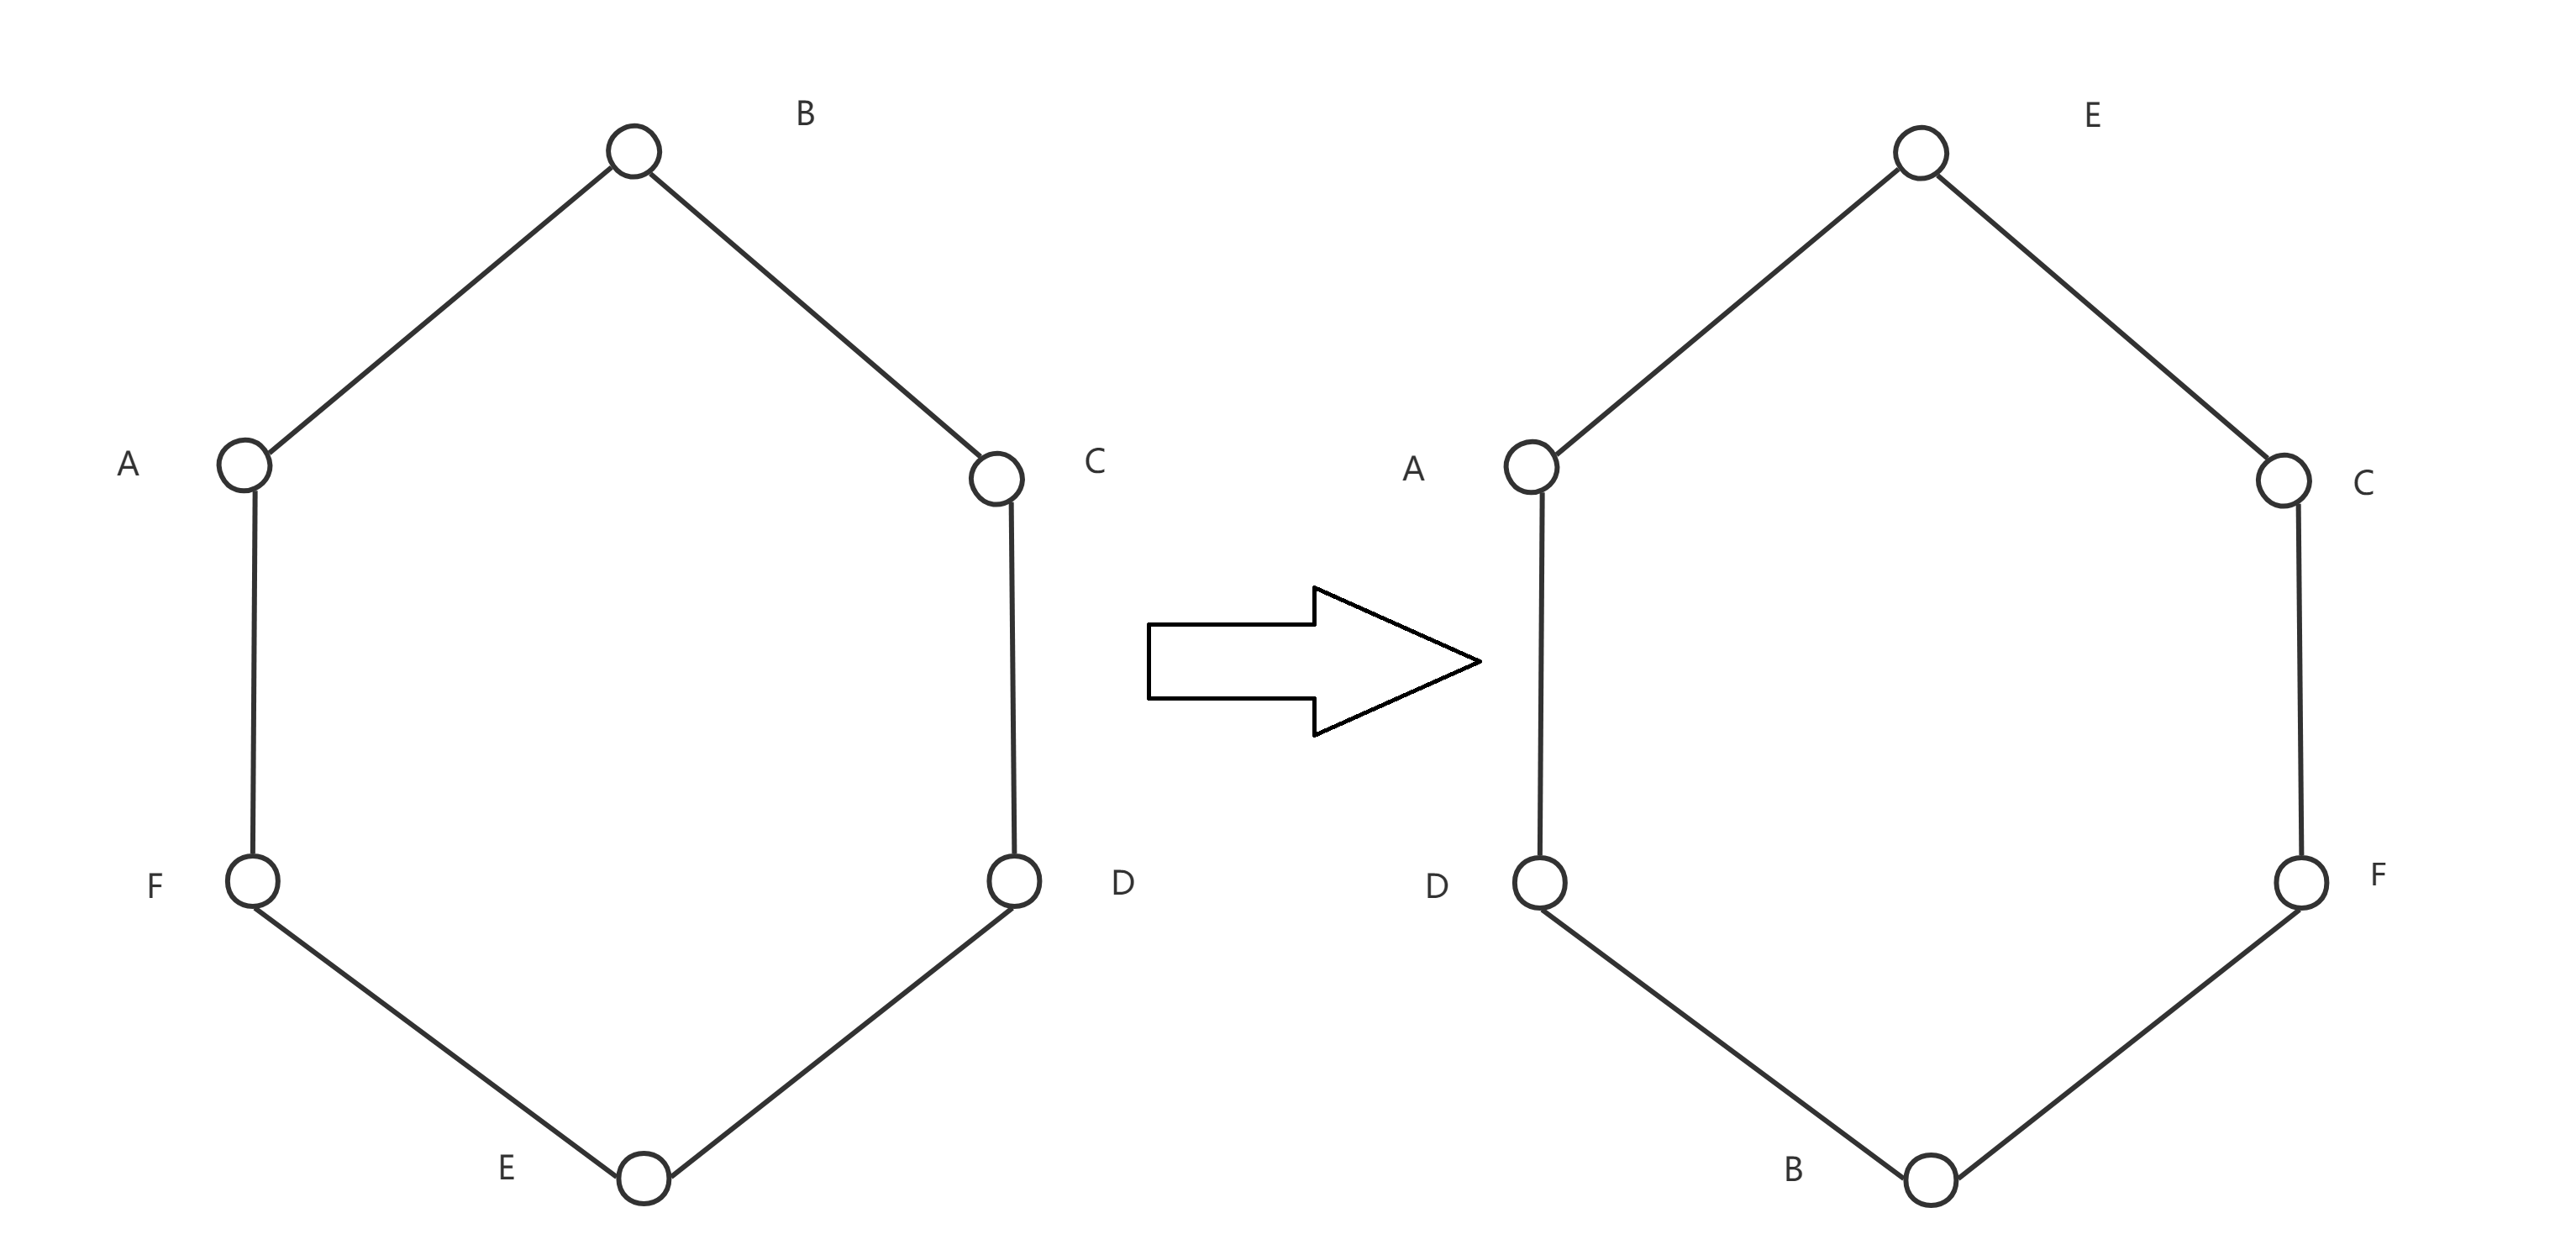
\includegraphics[scale=0.25]{t19.png}
\end{figure*}

\subsection*{20.}
    做$\nu$阶无向简单图$G=<V,E>$,其中$V=\{v|\ v\mbox{为人群中的成员}\}$,$E=\{uv|\ u,v\in V,\ u\neq v\mbox{且}u,\ v\mbox{相互认识}\}$,则
    \[
        \forall\ u,\ v\in V,\ \deg(u)+\deg (v)\geq \nu -2.
    \]
    对于不相邻的顶点$u,\ v$,若$\exists\ w\in V,\ w\neq u,w\neq v,\mbox{且} wu,wv$有一不属于$E$ (不妨设$wu\notin E$),则
    \[
        w,v\mbox{合起来认识的人不包括}u \ \Rightarrow\ \mbox{矛盾}.
    \]
    即
    \[
        \deg(u)+\deg (v) \geq 2(\nu-2).
    \]
    当$\nu \geq 3$时,有
    \[
        2(\nu -2)\geq \nu -1\ \Rightarrow\ G\mbox{有}Hamilton\mbox{轨道}.
    \]
    当$\nu \geq 4$时,有
    \[
        2(\nu -2)\geq \nu\ \Rightarrow\ G\mbox{有}Hamilton\mbox{圈}.
    \]
    将人群按$Hamilton$轨道及$Hamilton$圈排列即为所求.
    
    \clearpage
\subsection*{22.}
\begin{enumerate}
    \item [(1)]
    \begin{enumerate}
        \item [$1^\circ$]从$a$出发,形成轨道$P_1 = a$.
        \item [$2^\circ$]从$V(G) - {a }$中,选取与$a$ 最近的顶点$d$.形成 $P_2=ad$.
        \item [$3^\circ$]从$V(G) - {a ,d }$中,选取与$d$ 最近的顶点$e$.形成$P_3=ade$.
        \item [$4^\circ$]从$V(G) - {a ,d,e }$中,选取与$e$ 最近的顶$b$.形成$P_4=abeb$.
        \item [$5^\circ$]从$V(G) - {a,d,e,b }$中,选取与$b$ 最近的顶点$c$.形成$P_5=abebc$.
        \item [$6^\circ$]得$Hamilton$ 圈,$H = adebca,\ W=26$.
    \end{enumerate}

    \item [(2)]
    \begin{enumerate}
        \item [$1^\circ$]求$G$ 的一颗最小生成树$T$.
        \begin{figure*}[htbp]
            \centering
            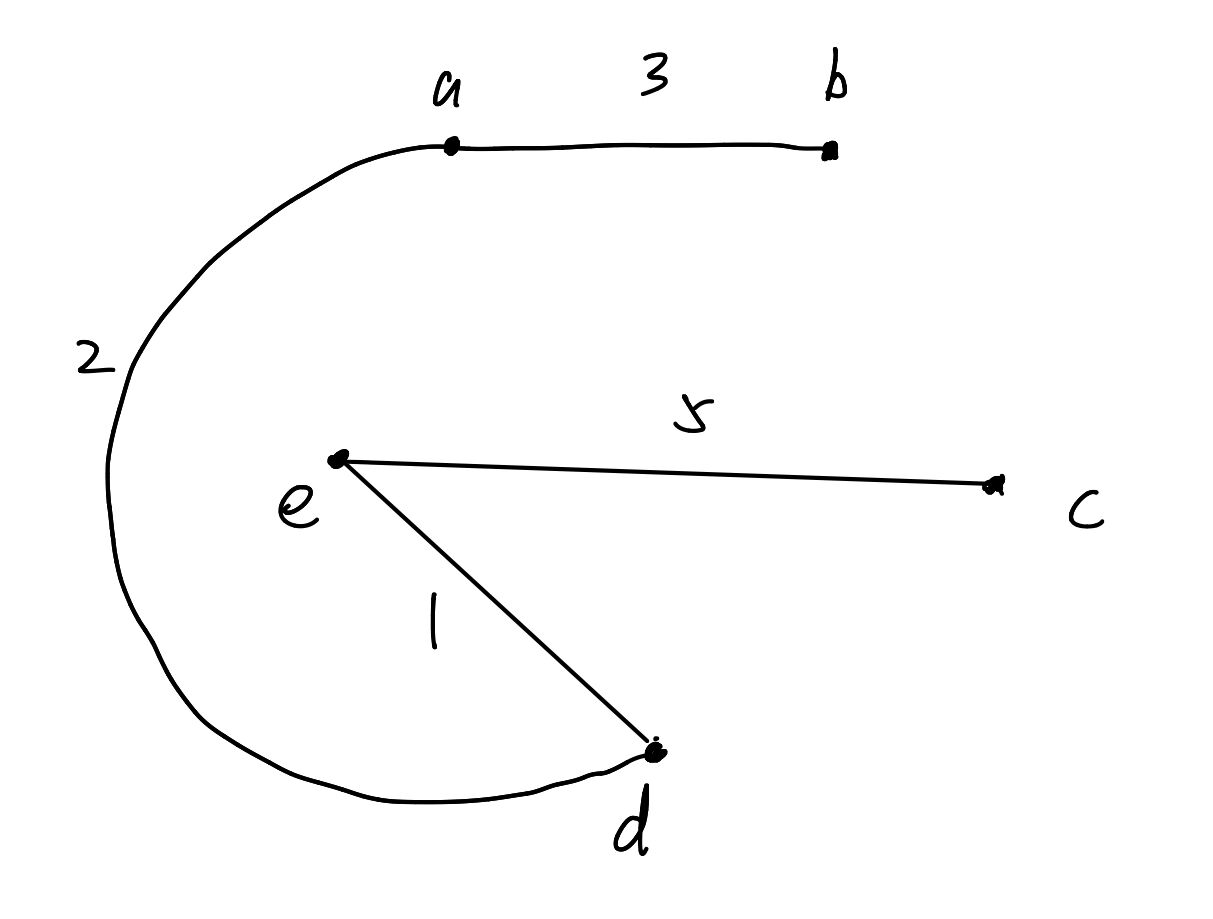
\includegraphics[scale=0.2]{t221.jpg}
        \end{figure*}
        \item [$2^\circ$]将$T$ 各边加平行边得$G^*$.
        \begin{figure*}[htbp]
            \centering
            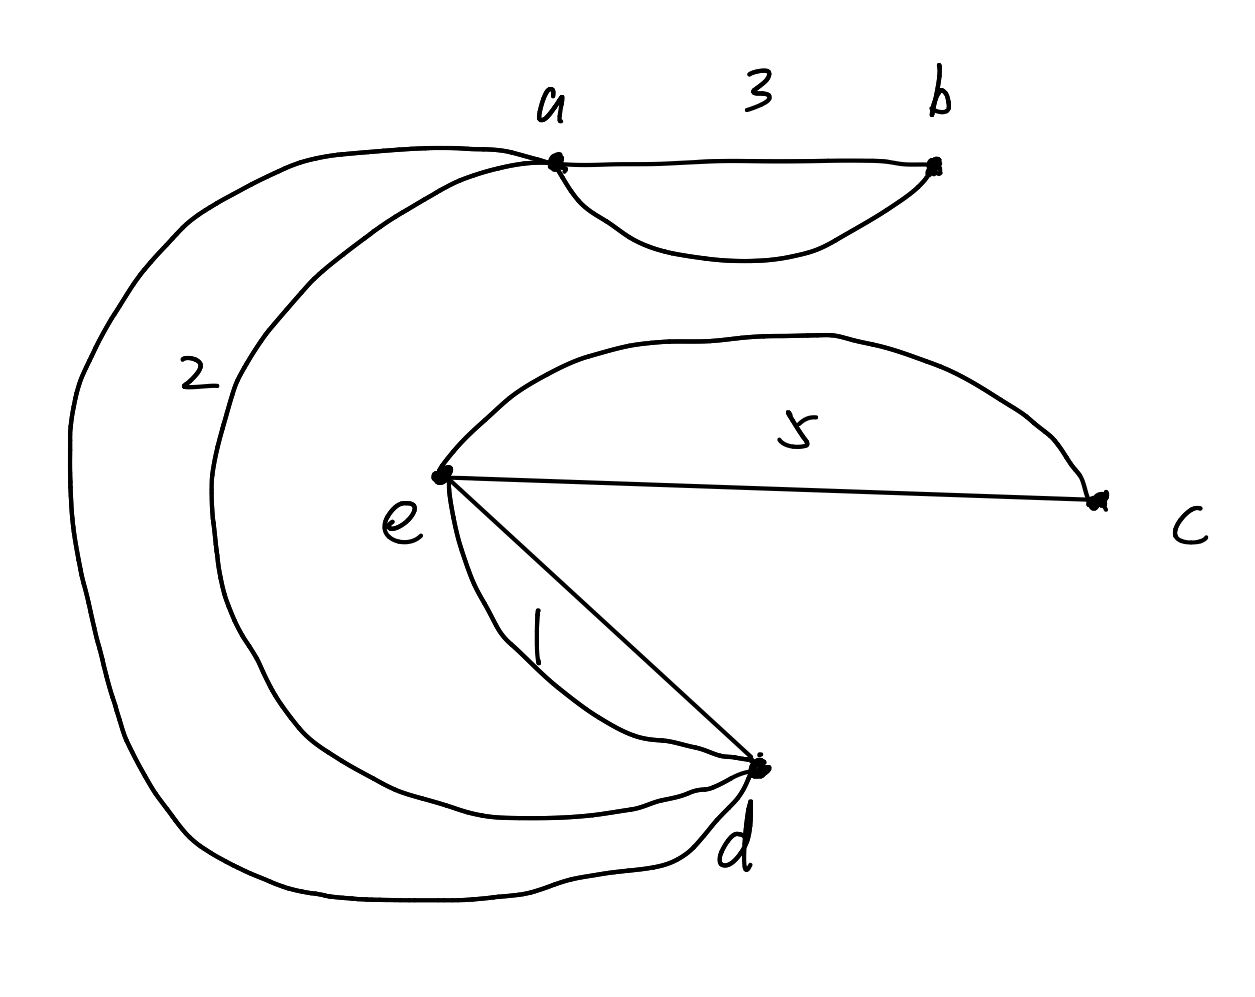
\includegraphics[scale=0.2]{t222.jpg}
        \end{figure*}
        \item [$3^\circ$]从$a$ 出发,求$G^* $ 的一条欧拉回路$C_a = adecedaba $ ,"抄近路" 访问$G$ 的各顶点。得$H_a = adecba,\ W_a=21$。
        \item [$4^\circ$]从$b$ 出发,求$G^* $ 的一条欧拉回路$C_b = badecedab $ ,"抄近路" 访问$G$ 的各顶点。得$H_b =badecb,\ W_b=21$。
    \end{enumerate}
    \clearpage
    \item [(3)]
    \begin{enumerate}
        \item [$1^\circ$]求$G$ 的一颗最小生成树$T$.
        \begin{figure*}[htbp]
            \centering
            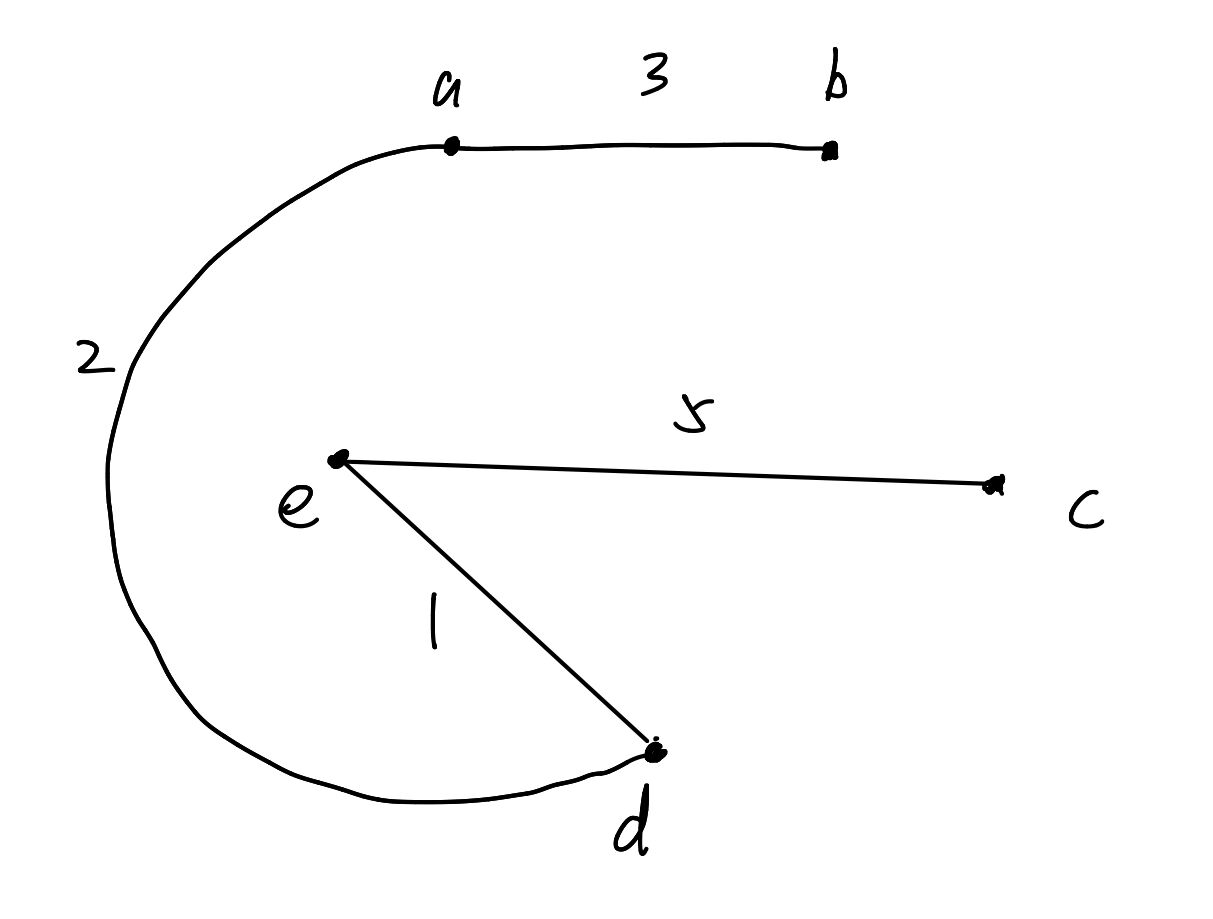
\includegraphics[scale=0.2]{t221.jpg}
        \end{figure*}
        \item [$2^\circ$] $T$中奇度数顶点得集合为$V_o = {b ,c }$, 
        $V_o$的导出子图中总权最小得完备匹配$M = {bc}$,$M$加入$T$中得$G*$.
        \begin{figure*}[htbp]
            \centering
            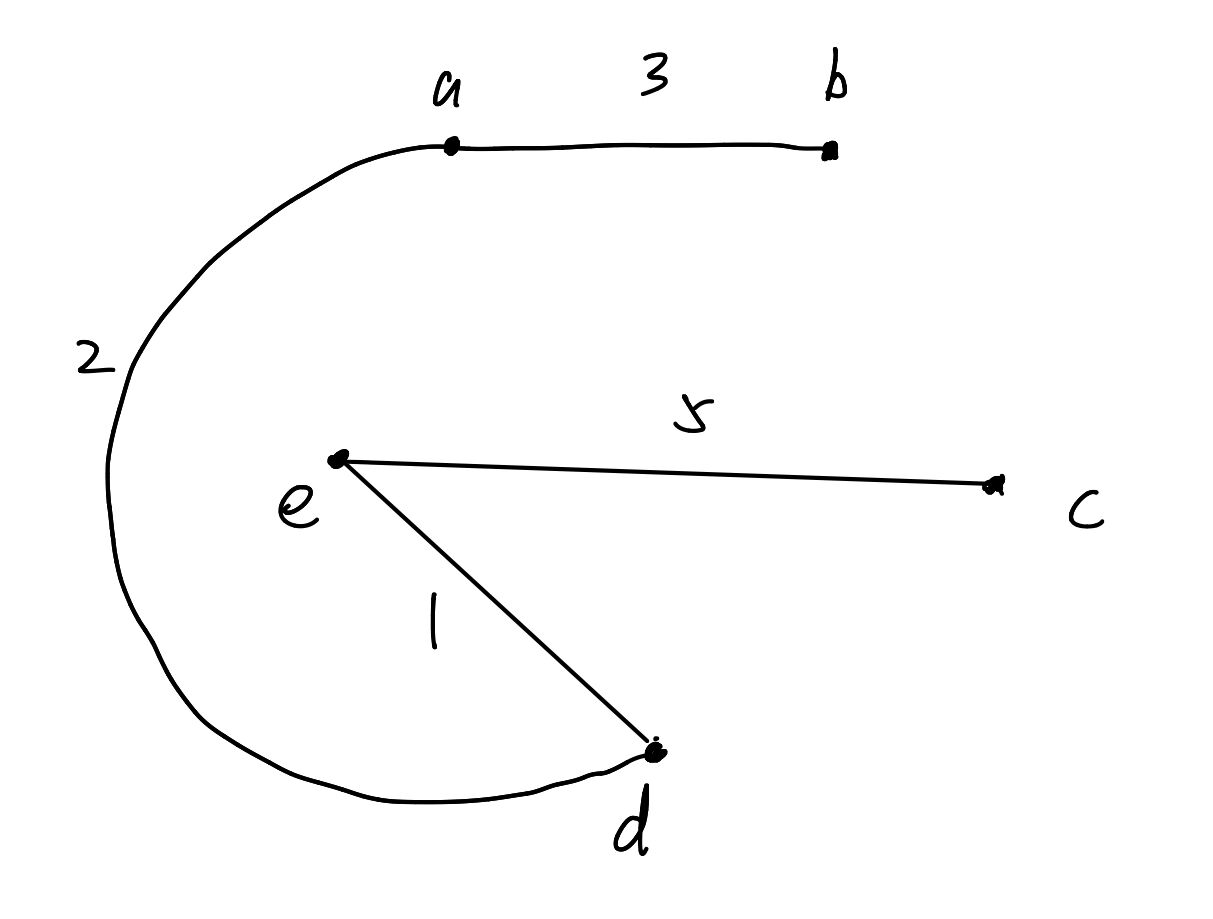
\includegraphics[scale=0.2]{t221.jpg}
        \end{figure*}

        \item [$3^\circ$]在$G^* $ 中求从$a$ 出发得一条欧拉回路$C_a =adecba $
        \item [$3^\circ$]在$G$ 中, 从$a$ 出发,沿$C_a$ 中得边按 ''抄近路'' 走出$Hamilton$ 圈$H_a = adecba$.
    \end{enumerate}
    $W=21$.
\end{enumerate}


\end{document}